% Options for packages loaded elsewhere
\PassOptionsToPackage{unicode}{hyperref}
\PassOptionsToPackage{hyphens}{url}
\PassOptionsToPackage{dvipsnames,svgnames*,x11names*}{xcolor}
%
\documentclass[
]{article}
\usepackage{lmodern}
\usepackage{amssymb,amsmath}
\usepackage{ifxetex,ifluatex}
\ifnum 0\ifxetex 1\fi\ifluatex 1\fi=0 % if pdftex
  \usepackage[T1]{fontenc}
  \usepackage[utf8]{inputenc}
  \usepackage{textcomp} % provide euro and other symbols
\else % if luatex or xetex
  \usepackage{unicode-math}
  \defaultfontfeatures{Scale=MatchLowercase}
  \defaultfontfeatures[\rmfamily]{Ligatures=TeX,Scale=1}
\fi
% Use upquote if available, for straight quotes in verbatim environments
\IfFileExists{upquote.sty}{\usepackage{upquote}}{}
\IfFileExists{microtype.sty}{% use microtype if available
  \usepackage[]{microtype}
  \UseMicrotypeSet[protrusion]{basicmath} % disable protrusion for tt fonts
}{}
\usepackage{xcolor}
\IfFileExists{xurl.sty}{\usepackage{xurl}}{} % add URL line breaks if available
\IfFileExists{bookmark.sty}{\usepackage{bookmark}}{\usepackage{hyperref}}
\hypersetup{
  colorlinks=true,
  linkcolor=blue,
  filecolor=Maroon,
  citecolor=Blue,
  urlcolor=Blue,
  pdfcreator={LaTeX via pandoc}}
\urlstyle{same} % disable monospaced font for URLs
\usepackage[margin=2.5cm]{geometry}
\usepackage{graphicx}
\makeatletter
\def\maxwidth{\ifdim\Gin@nat@width>\linewidth\linewidth\else\Gin@nat@width\fi}
\def\maxheight{\ifdim\Gin@nat@height>\textheight\textheight\else\Gin@nat@height\fi}
\makeatother
% Scale images if necessary, so that they will not overflow the page
% margins by default, and it is still possible to overwrite the defaults
% using explicit options in \includegraphics[width, height, ...]{}
\setkeys{Gin}{width=\maxwidth,height=\maxheight,keepaspectratio}
% Set default figure placement to htbp
\makeatletter
\def\fps@figure{htbp}
\makeatother
\setlength{\emergencystretch}{3em} % prevent overfull lines
\providecommand{\tightlist}{%
  \setlength{\itemsep}{0pt}\setlength{\parskip}{0pt}}
\setcounter{secnumdepth}{-\maxdimen} % remove section numbering
\newlength{\cslhangindent}
\setlength{\cslhangindent}{1.5em}
\newenvironment{cslreferences}%
  {\setlength{\parindent}{0pt}%
  \everypar{\setlength{\hangindent}{\cslhangindent}}\ignorespaces}%
  {\par}

\title{
\includegraphics[width=4cm,height=\textheight]{logoUMAG.jpg}}
\author{}
\date{\vspace{-2.5em}}

\begin{document}
\maketitle


\pagenumbering{gobble}

%\begin{titlepage}
\begin{flushleft}
\Large{\textbf{Ensayo Científico}}\\
\vspace*{2\baselineskip}
\LARGE{\textbf{Forzantes del Cambio Climático y su impacto en las poblaciones marinas del Océano Austral}}\\
\vspace*{3\baselineskip}
\Large{Curso Cambio Climático}\\
\Large{Semestre-1 2021 }\\
\vspace*{4\baselineskip}
\end{flushleft}
\begin{flushright}
\large{\textbf{Mauricio Mardones Inostroza}}\\
\vspace*{2\baselineskip}
\normalsize{Alumno Programa de Doctorado Ciencias Antárticas y Sub-Antárticas}\\
\vspace*{1\baselineskip}
\normalsize{Universidad de Magallanes, Chile}\\
\vspace*{1\baselineskip}
\normalsize{\textbf{Profesores}}\\
Dr. Rodrigo Villa-Martinez\\
Dr. Juan Carlos Aravena\\
\vspace*{1\baselineskip}
\normalsize{\textbf{Fecha}}\\
Mayo, 2021
\end{flushright}

% \end{titlepage}


\hypersetup{linkcolor = black}
\newpage
\pagenumbering{roman}
%\tableofcontents
%\addcontentsline{toc}{section}{\contentsname}

\newpage



\pagenumbering{arabic}
\hypersetup{linkcolor = blue}

\fontsize{12}{26}
\selectfont{}

\hypertarget{introduccion}{%
\subsection{1. INTRODUCCION}\label{introduccion}}

En las últimas décadas, las evidencias de los cambios en variables
climáticas y oceanográficas están demostradas con profusa evidencia
científica las cuales han sido bien compiladas por el Panel
Intergubernamental sobre Cambio Climático (IPCC por sus siglas en
inglés) (IPCC, \protect\hyperlink{ref-IPCC2014}{2014}). El impacto de
estos cambios se ha traducido en perturbaciones en estructura y
funcionamiento de los ecosistemas y han sido asociados a la acción
antropogénica (Worm et al., \protect\hyperlink{ref-Worm2012}{2012}) y
relativos al Cambio Climático (CC) global (Bryndum-Buchholz et al.,
\protect\hyperlink{ref-Bryndum-Buchholz2019}{2019}; Rijnsdorp et al.,
\protect\hyperlink{ref-Rijnsdorp2009}{2009}).

Un forzante (o \emph{driver}) se define como cualquier factor natural o
antropogénico que causa cambios directos o indirectos en un ecosistema.
Un forzante directo tiene influencia inéquivoca sobre los procesos
ecosistémicos, por otro lado, un forzante indirecto opera de forma
difusa, por alteración de uno o mas forzantes. En las poblaciones
marinas, los forzantes directos tienen impacto sobre la fisiología y
aspectos fenológicos, y los forzantes indirectos tienen impacto sobre la
productividad primaria o interacciones ecológicas, distribución espacial
o transporte larval (Koenigstein et al.,
\protect\hyperlink{ref-Koenigstein2016}{2016}).

En todos los océanos del mundo, las poblaciones marinas están
evidenciando los efectos del CC, ya sea por la suma y/o combinación de
los forzantes del CC, y sobre lo cual existe sólida evidencia científica
que demuestra los efectos en respuestas como fisiología, ecología y
variables observables como distribución, biomasas y productividad en
escalas locales y globales (Barange et al.,
\protect\hyperlink{ref-Barange2014}{2014}; Bryndum-Buchholz et al.,
\protect\hyperlink{ref-Bryndum-Buchholz2019}{2019}; Perry et al.,
\protect\hyperlink{ref-Perry2005}{2005}; Rijnsdorp et al.,
\protect\hyperlink{ref-Rijnsdorp2009}{2009}). Estas nuevas condiciones
externas están produciendo impactos en los ecosistemas marinos a través
de cambios en los hábitats (Bryndum-Buchholz et al.,
\protect\hyperlink{ref-Bryndum-Buchholz2019}{2019}; Hidalgo et al.,
\protect\hyperlink{ref-Hidalgo2018}{2018}; Rijnsdorp et al.,
\protect\hyperlink{ref-Rijnsdorp2009}{2009}; Shoji et al.,
\protect\hyperlink{ref-Shoji2011}{2011}), lo cual tiene efectos en la
sustentabilidad de las poblaciones y a su vez, en los sistemas
socio-ecológicos asociados.

Existen múltiples evidencias que demuestran y cuantifican el impacto del
CC en distintos grupos de especies marinas, ya sean estas; mamíferos,
peces, moluscos y diversos organismos que constituyen comunidades
ecológicas en distintos ecosistemas del planeta. Algunos autores
proponen que los impactos del CC, a través de un calentamiento de las
masas de agua, gatillaría cambios en los patrones de distribución
espacial de los organismos marinos haciéndolos migrar hacia altas
latitudes (Cheung et al., \protect\hyperlink{ref-Cheung2010a}{2010};
Kortsch et al., \protect\hyperlink{ref-Kortsch2015}{2015};
Melbourne-Thomas et al.,
\protect\hyperlink{ref-Melbourne-Thomas2021}{2021}). En este sentido, es
necesario entender cómo impactarán estos forzantes ambientales en
ecosistemas de altas latitudes como, por ejemplo, el Oceano Austral
(OA), y por ende, cómo responderán las especies marinas que allí
habitan. En ese sentido, regiones polares deben ser analizadas a la luz
de la evidencia científica, identificando los cambios ocurridos, así
como también, proyectar los impactos del CC en estas poblaciones.

El Océano Austral que rodea la Antártica, es un componente crítico del
sistema terrestre, y sustenta un ecosistema marino de inmenso valor
ecológico, económico e intrínseco. Este océano está definido
espacialmente en función de la Corriente Circumpolar Antártica, la que
más agua transporta en todo el océano. Esta corriente formada hace 34
millones de años fluye casi libremente de oeste a este alrededor del
continente Antártico, en una banda fluctuante que se ubica
aproximadamente en los 60º de latitud sur. En este punto el agua es más
fría y menos salada que en los océanos colindantes. Por todas estas
caracteristicas, este océano es una de los áreas más sensibles al CC.
Los forzantes claves y su influencia en procesos claves dentro del OA ya
han experimentado cambios en sus atributos, entre ellos se pueden
identificar; la temperatura del océano, la dinámica del hielo marino, la
estratificación, las corrientes, entre otros (Morley et al.,
\protect\hyperlink{ref-Morley2020}{2020}; Sylvester et al.,
\protect\hyperlink{ref-Sylvester2021}{2021}).

En el OA habitan especies que conforman las mas grandes poblaciones
marinas del planeta, entre ellas el krill \emph{Euphausia superba} y
peces demersales como el bacalao antártico \emph{Dissostichus mawsoni}
(Atkinson et al., \protect\hyperlink{ref-Atkinson2009}{2009}; Piñones \&
Fedorov, \protect\hyperlink{ref-Pinones2016}{2016}; Veytia et al.,
\protect\hyperlink{ref-Veytia2020}{2020}). Estas dos especies son
esenciales en el Océano Austral, dado que forman parte estructural de la
red trófica y ecológica (Atkinson et al.,
\protect\hyperlink{ref-Atkinson2009}{2009}; Piñones \& Fedorov,
\protect\hyperlink{ref-Pinones2016}{2016}). Por otro lado, estas
poblaciones son explotadas intensamente por la industria pesquera desde
hace más de 50 años, constituyendo una actividad económica muy
importante. En este sentido, cualquier impacto que tengan los distintos
forzantes ambientales sobre la productividad de estas especies marinas
concita múltiples intereses, que van desde lo científico hasta lo
económico.

Entender entonces cuales son y como actuan los principales forzantes y
su impacto en los procesos poblacionales de las especies mas importantes
que habitan el OA y como estas especies responderán a esta influencia es
fundamental para comprender y anticiparse a algun escenario climático.
El objetivo por tanto es identificar la influencia del CC a través de
los forzantes ambientales en las poblaciones marinas más importantes del
Océano Austral.

\pagebreak

\hypertarget{desarrollo}{%
\subsection{2. DESARROLLO}\label{desarrollo}}

Cualquier percepción de un ambiente marino sin cambios es hoy en día una
afirmación ingenua y sesgada. Esta mirada se contradice fácilmente
observando las dramáticas evidencias de cambios en la estructura,
abundancia y distribución de las especies a través de la escala temporal
desde años, décadas, siglos y milenios (Pinsky et al.,
\protect\hyperlink{ref-Pinsky2020}{2020}). En este sentido, es
importante determinar qué forzantes ambientales están produciendo los
cambios a nivel poblacional. Este tipo de estudios han sido abundantes
en este último tiempo dada la importancia del OA y las poblaciones que
allí habitan en un contexto de CC acelerado.

Morley et al. (\protect\hyperlink{ref-Morley2020}{2020}) han clasificado
los forzantes mas importantes y con mayor influencia en el OA, los
cuales se clasifican como forzantes físicos, antropogénicos y
biológicos. Entre los forzantes físicos, se pueden identificar el
calentamiento global, procesos atmosférico-oceanográficos y corrientes
marinas.

Respecto a los forzantes asociados al calentamiento global que tienen
impacto en las poblaciones marinas, los factores con más evidencias son
la temperatura y el oxígeno disuelto. Estos dos forzantes son los
principales responsables de control del metabolismo aeróbico de
organismos ectotermos como peces y crustáceos, y son también los dos
variables ambientales influenciadas de manera más generalizada por
cambio climático de origen antropogénico (Duncan et al.,
\protect\hyperlink{ref-Duncan2020}{2020}).

\hypertarget{temperatura}{%
\subsection{2.1. Temperatura}\label{temperatura}}

La temperatura regula la tasa de metabolismo aeróbico a través del
consumo de energía para procesos fisiológicos, proceso acelerado cuando
el organismo está sometido a altas temperaturas. En este sentido, cabe
señalar que el océano se ha calentado sin cesar desde 2005, mostrando
claras tendencias bien documentadas en el 5to Reporte de Evaluación del
IPCC (IPCC, \protect\hyperlink{ref-IPCC2014}{2014}). La tendencia de
calentamiento se ve confirmada por las mediciones de la temperatura del
océano durante la última década. Las profundidades de 0-700 m. y
700-2000 m. del océano se han calentado a tasas de 5,31 ± 0,48 y 4,02 ±
0,97 gº año-1 de 2005 a 2017. La tendencia a largo plazo para
profundidades de 0-700 m. y 700-2000 m. se han calentado 4,35 ± 0,8 y
2,25 ± 0,64 gº año-1 entre 1971-1990 y 1998-2017 respectivamente. Es
probable que el calentamiento del océano haya continuado en el océano
abisal y profundo por debajo de los 2000 m (hemisferio sur y océano
austral) (Bindoff et al., \protect\hyperlink{ref-Bindoff2019}{2019}).

Con respecto a la temperatura y a sus variaciones futuras,
Bryndum-Buchholz et al.
(\protect\hyperlink{ref-Bryndum-Buchholz2019}{2019}) realizaron
predicciones por medio de simulaciones de biomasas de peces en distintos
océanos a través de modelos de ensamble, y se identificaron diferentes
resultados frente a la misma variable ambiental, que en este caso fue la
variabilidad de la Temperatura Superficial del Mar (TSM) (Figura 1).

Cabe destacar de acuerdo a este análisis, que en la gran mayoría de los
océanos, la relación entre el aumento de TSM y cambios en biomasa fueron
inversamente proporcionales, salvo para los océanos Austral y Ártico, en
donde los cambios en la temperatura beneficiarían a las poblaciones
marinas de aquellos ecosistemas. Estos resultados coinciden con lo
propuesto por Koenigstein et al.
(\protect\hyperlink{ref-Koenigstein2016}{2016}), quienes apuntaban a
beneficios en las poblaciones marinas de ecosistemas de altas latitudes
por efecto del CC y el calentamiento global.

\pagebreak

\begin{figure}

{\centering 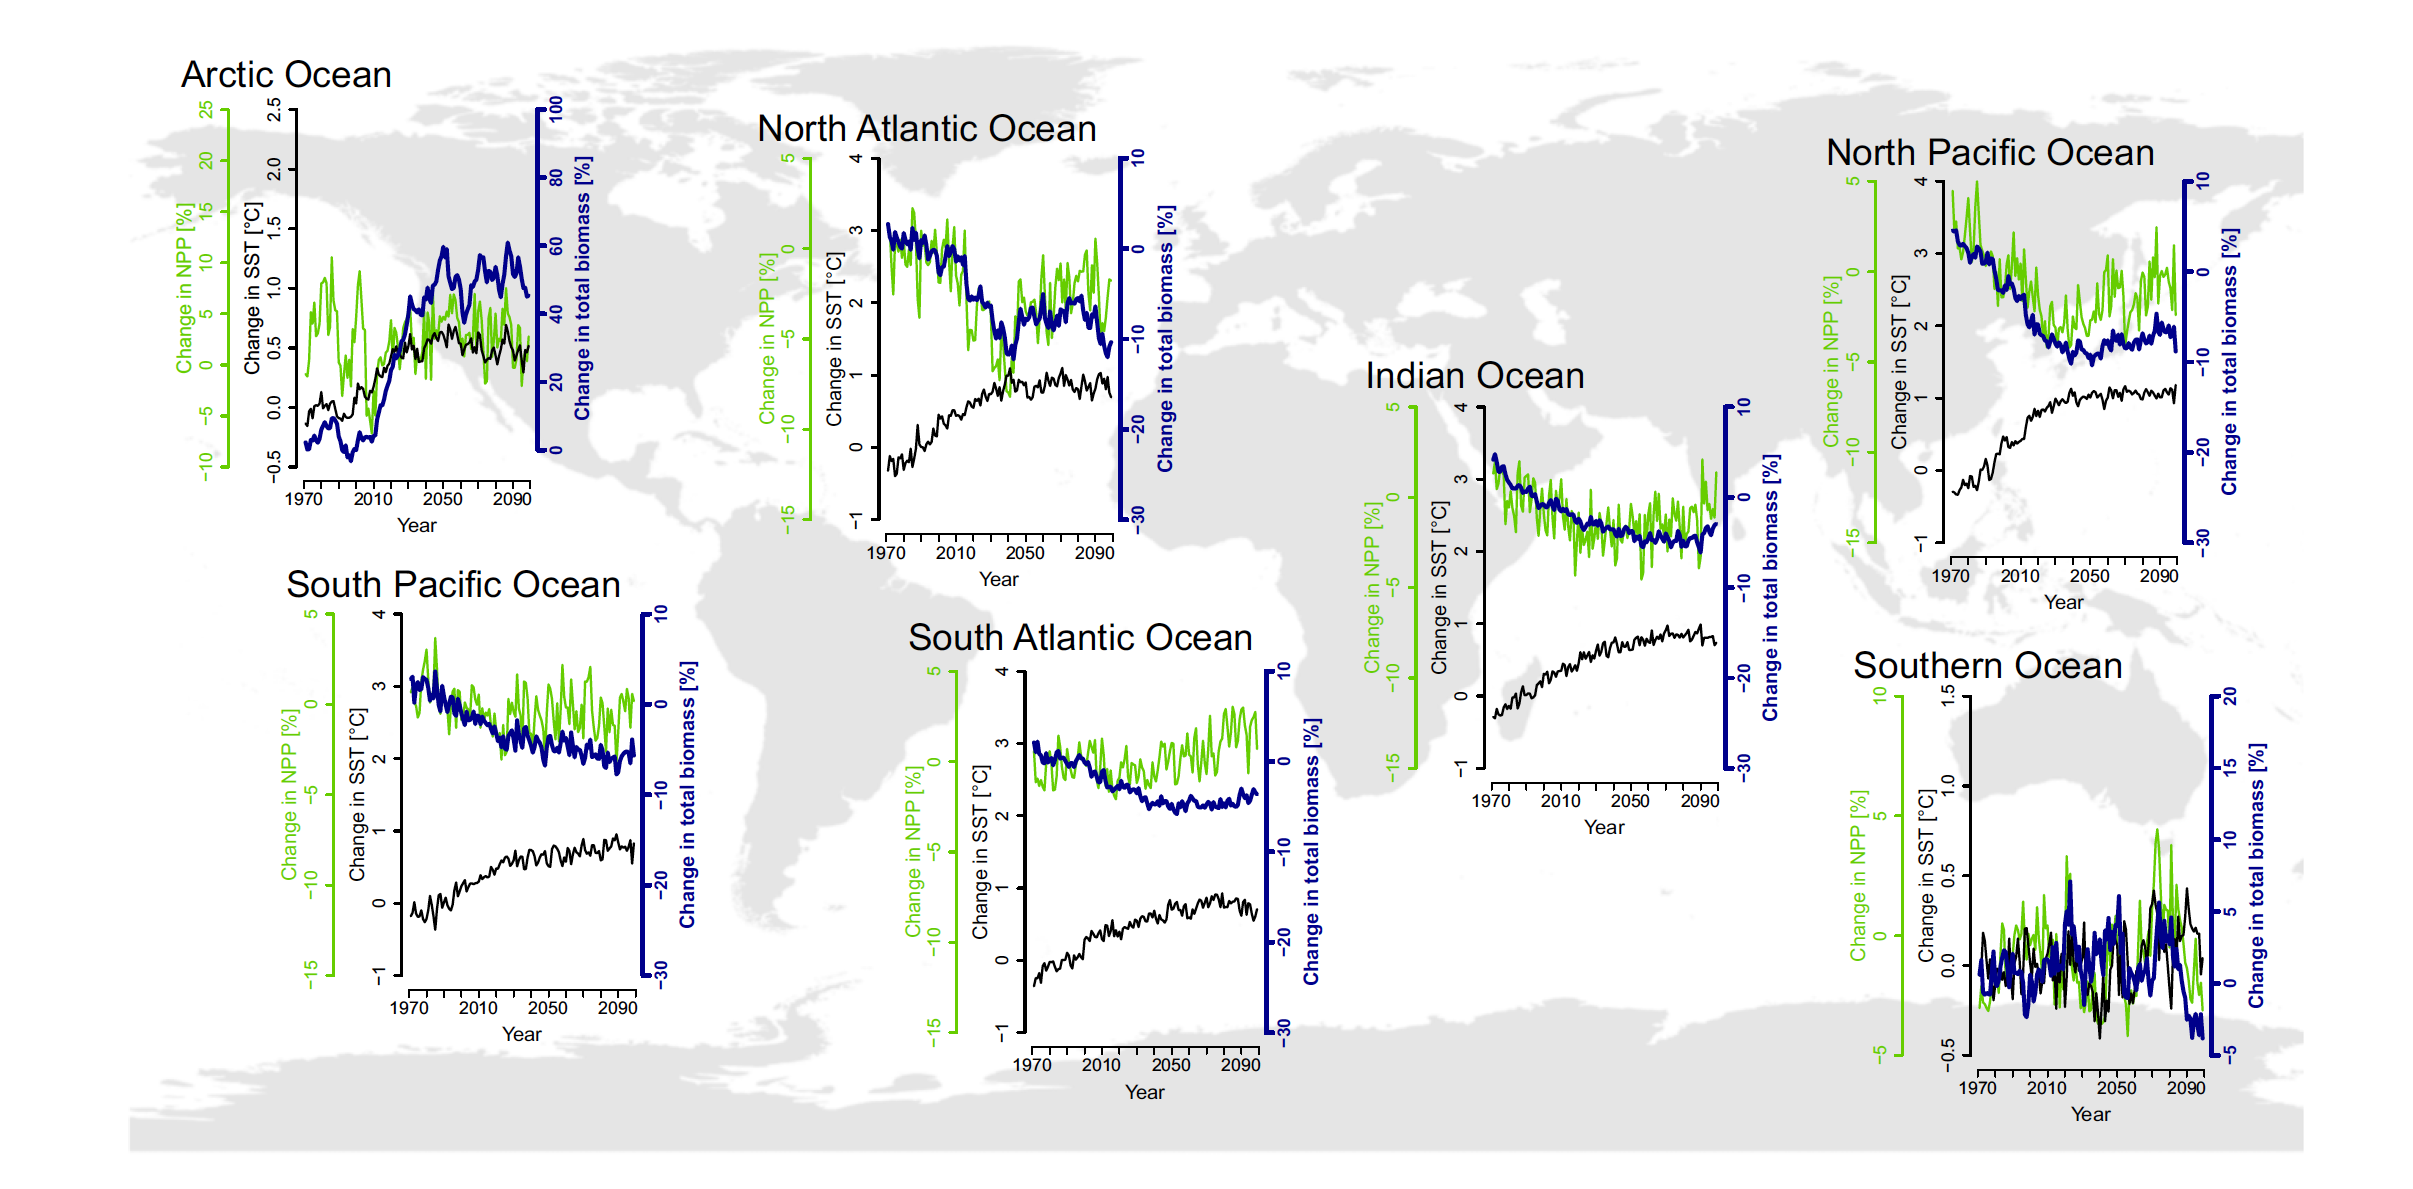
\includegraphics[width=1\linewidth]{images/Exa} 

}

\caption{Proyección de los impactos de Cambios Climáticos en indicadores poblacionales de especies marinas alrededor del mundo (Bryndum-Buchholz et al,. 2019)}\label{fig:unnamed-chunk-1}
\end{figure}

Rijnsdorp et al. (\protect\hyperlink{ref-Rijnsdorp2009}{2009}) indican
que la temperatura tiene un efecto directo sobre la fisiología, el
crecimiento, la reproducción, el reclutamiento y el comportamiento de
organismos poiquilotérmicos como los peces, moluscos, cefalópodos y
crustáceos. También identifican que la temperatura tendrá un efecto
sobre aspectos de la historia de vida y ontogenia de las especies, en
donde, diferentes estadíos de un organismo (huevos, larvas, juveniles,
adultos) pueden ser influidos por la temperatura de forma distinta
(Figura 2).

\pagebreak

\begin{figure}

{\centering 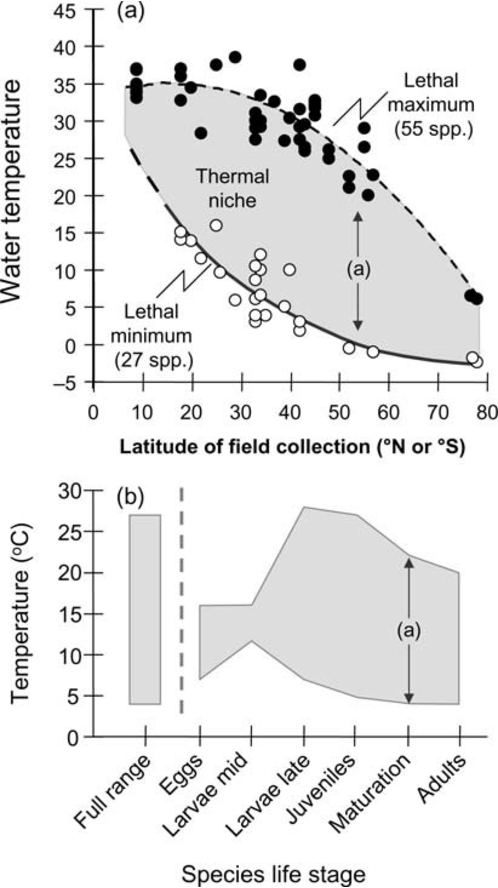
\includegraphics[width=0.5\linewidth]{images/Exa17} 

}

\caption{Diagrama conceptual de los cambios en los hábitats óptimos (basado en la temperatura del agua) con (a) latitud de la especie y/o población y (b) por etapa de vida. La flecha (a) denota un rango de temperaturas tolerables medidas para adultos durante la maduración y desove. (Rijnsdorp et al., 2009)}\label{fig:unnamed-chunk-2}
\end{figure}

De acuerdo también a estos resultados, es posible identificar un rango
de tolerancia a la temperatura (nicho termal) muy estrecho en altas y
bajas latitudes y con un amplio rango de tolerancia en latitudes
intermedias (Figura 2.

El cambio de la temperatura del medio marino afecta a muchos procesos
fisiológicos que van desde dañar las proteínas hasta alterar la función
de los órganos. Los cambios ambientales, especialmente el calentamiento
global, pueden por tanto influir fuertemente en la abundancia y
distribución de los peces a través de umbrales fisiológicos específicos
de especies de tolerancia a la temperatura, o mediante respuestas a
cambios en otros niveles tróficos (Perry et al.,
\protect\hyperlink{ref-Perry2005}{2005}; Rijnsdorp et al.,
\protect\hyperlink{ref-Rijnsdorp2009}{2009}; Saba et al.,
\protect\hyperlink{ref-Saba2014}{2014}). En este contexto, los cambios
en el rango de distribución espacial de los organismos marinos se
encuentran entre las consecuencias más perceptibles del cambio climático
a escala mundial, con impactos potencialmente significativos en la pesca
comercial (Barange et al., \protect\hyperlink{ref-Barange2014}{2014};
Perry et al., \protect\hyperlink{ref-Perry2005}{2005}), en las redes
tróficas y el funcionamiento de los ecosistemas y sobre la biodiversidad
en su conjunto (Pinsky et al.,
\protect\hyperlink{ref-Pinsky2020}{2020}).

Los organismos marinos responden al aumento de la temperatura del océano
a través de cambios de distribución, con cambios regionales esperados
hacia aguas más frías, más profundas, más marinas o polares, así como
también en el rango global (Cheung et al.,
\protect\hyperlink{ref-Cheung2010a}{2010}; Frawley et al.,
\protect\hyperlink{ref-Frawley2019}{2019}; Pinsky et al.,
\protect\hyperlink{ref-Pinsky2020}{2020}).

Las temperaturas locales en los ecosistemas marinos polares están
aumentando dos veces más rápido que el promedio mundial (IPCC,
\protect\hyperlink{ref-IPCC2014}{2014}), lo que lleva a una
borealización de las comunidades de animales del Ártico, con una
disminución de la abundancia de especies con afinidad polar y abundancia
creciente de especies boreales. Se espera que la abundancia general de
especies en mares semicerrados (es decir, el mar Mediterráneo, el mar
Báltico) y las cuencas oceánicas tropicales disminuya en el futuro
(Cheung et al., \protect\hyperlink{ref-Cheung2013}{2013}).

\pagebreak

\hypertarget{oxuxedgeno-disuelto}{%
\subsection{2.2. Oxígeno disuelto}\label{oxuxedgeno-disuelto}}

Por su parte, la disponibilidad de oxígeno plantea un límite superior en
el metabolismo aeróbico, en la cual un organismo puede consumir el
oxígeno requerido para alimentar los procesos fisiológicos. Este se
establece mediante tasas de difusión a través de un gradiente de presión
desde medio ambiente (Duncan et al.,
\protect\hyperlink{ref-Duncan2020}{2020}).

Recientemente se demostró que el tamaño del cuerpo de los peces puede
reducirse debido al cambio climático, especialmente en respuesta al
calentamiento, la reducción del oxígeno y la disponibilidad de recursos
(Cheung et al., \protect\hyperlink{ref-Cheung2013}{2013}). El IPCC
proyecta que los océanos se volverán más cálidos y menos oxigenados
(IPCC, \protect\hyperlink{ref-IPCC2014}{2014}).

El cambio climático está disminuyendo las concentraciones de oxígeno en
el mar abierto (Deutsch et al.,
\protect\hyperlink{ref-Deutsch2015}{2015}; Isensee et al.,
\protect\hyperlink{ref-Isensee2016}{2016}). Los efectos combinados del
cambio climático y exceso de nutrientes (nitrógeno y fósforo de fuentes
como la escorrentía agrícola y los desechos humanos) están conduciendo a
disminuciones de oxígeno en sistemas marinos costeros y mares
semicerrados que están fuertemente influenciados por su línea divisoria
de aguas en un contexto global y regional. Los modelos predicen que el
contenido de oxígeno en los océanos continúan disminuyendo a medida que
las temperaturas atmosféricas y oceánicas aumenta y aumenta el tamaño de
la población humana (Isensee et al.,
\protect\hyperlink{ref-Isensee2016}{2016}).

En este sentido, los impactos producidos por los cambios en las
concentraciones del oxígeno disuelto en el mar se traducen en una
modulación importante en las poblaciones marinas y su funcionamiento. La
evidencia reciente sugiere que los efectos combinados del calentamiento
y la pérdida de oxígeno juntos limitan las distribuciones geográficas de
organismos ectotermos marinos (Deutsch et al.,
\protect\hyperlink{ref-Deutsch2015}{2015}; Isensee et al.,
\protect\hyperlink{ref-Isensee2016}{2016}; Pörtner,
\protect\hyperlink{ref-Portner2001}{2001}). Se necesita suficiente
oxígeno para que un organismo pueda sobrevivir, alimentarse, defenderse,
crecer y reproducirse. Con el calentamiento esperado para finales de
siglo, las pérdidas de hábitat serán particularmente agudas en los
límites hacia el ecuador (Deutsch et al.,
\protect\hyperlink{ref-Deutsch2015}{2015}). Estos resultados sugieren
que es probable que los impactos sinérgicos tanto del oxígeno como del
calentamiento, moldeen fuertemente las distribuciones de especies
futuras, la biomasa, producción y función del ecosistema.

Los límites de los rangos de tolerancia térmica desde el ecuador, a
menudo coinciden con los hábitats donde el suministro de oxígeno es de
dos a cinco veces la demanda de oxígeno establecida por la tasa
metabólica en reposo de una especie (Deutsch et al.,
\protect\hyperlink{ref-Deutsch2015}{2015}). Por otro lado, y de acuerdo
a las proyecciones del IPCC, los océanos llegarán a tener aguas más
tibias y menos oxígeno disuelto (IPCC,
\protect\hyperlink{ref-IPCC2014}{2014}), dado que las temperaturas más
cálidas impulsan tasas metabólicas más altas, las que superan la
disponibilidad de oxígeno. Un ejemplo de esto, fue identificado en el
Mar Mediterráneo, en donde Cheung et al.
(\protect\hyperlink{ref-Cheung2013}{2013}) usaron un Modelo Envolvente
de Bioclima Dinámico, el cual simuló cambios en la abundancia relativa y
distribución espacial de poblaciones marinas en una grilla global,
considerando aspectos ecofisiológicos, preferencias y tolerancias a
condiciones ambientales y movimiento de individuos adultos. En este
analisis se determinó que el peso promedio de los peces disminuyó entre
un 4\% a un 49\% desde el 1970 al 2050 (Figura 3).

\newpage

\begin{figure}

{\centering 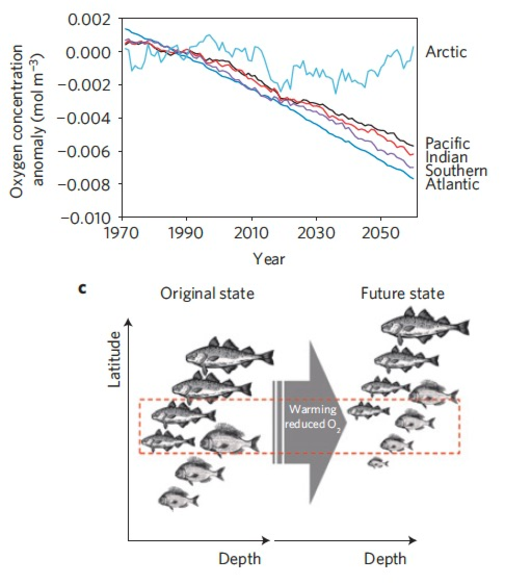
\includegraphics[width=1\linewidth]{images/Exa18} 

}

\caption{Proyección de las condiciones climáticas y las esperadas respuestas biológicas de peces en términos de tamaño y peso. Panel superior indica concentración de oxígeno disuelto proyectado. Panel inferior muestra una visión esquemática de los cambios esperados en las comunidades marinas en función del oxígeno disuelto (Cheung et al., 2013)}\label{fig:unnamed-chunk-3}
\end{figure}

Sin embargo, estos estudios deben ser analizados en detalle, dado que
proyectar escenarios futuros de oxígeno disuelto es una tarea
arriesgada. No hay consenso sobre el volumen futuro de aguas con poco
oxígeno en mar abierto debido a las grandes incertidumbres sobre los
posibles efectos biogeoquímicos y la evolución de la dinámica de los
océanos tropicales (IPCC, \protect\hyperlink{ref-IPCC2014}{2014}).

\hypertarget{samenso}{%
\subsection{2.3. SAM/ENSO}\label{samenso}}

Existen forzantes globales que afectan al OA en el presente y también
afectarán en el futuro. Forzantes atmosférico-oceanógraficos son los que
se manifiestan por cambios producidos en la atmósfera y que tienen
implicancias en el mar, como por ejemplo, el Southern Annular Mode (SAM)
y El Niño Southern Oscillation (ENSO).

El agotamiento del ozono influye directamente en el modo principal de
variabilidad de la circulación atmosférica en las regiones
extratropicales del sur. Este fenómeno climático es llamado Modo Anular
del SUR o Southern Annular Mode (SAM, por sus siglas en inglés). Una
forma de medir el SAM es a través de un índice calculado como el
gradiente de presión entre las latitudes medias y la Antártida, que
cuando es muy positivo, da como resultado vientos del oeste que son más
fuertes que el promedio y se desplazan hacia el polo. Desde 1957 ha
habido un aumento significativo de la fase SAM positivo en el verano y
otoño austral. Se cree que la tendencia del verano se debe
principalmente al agotamiento del ozono polar estratosférico. La
variabilidad del SAM tiene un impacto significativo en la temperatura de
la superficie antártica, la precipitación y el hielo marino (Marshall et
al., \protect\hyperlink{ref-Marshall2018}{2018}).

Saba et al. (\protect\hyperlink{ref-Saba2014}{2014}) estudiarón los
efectos del clima a gran escala y el forzamiento físico producido por
distintas fases del SAM sobre los procesos biológicos en Península
Antártica. En este estudio identificaron los impactos de las fases
estacionales del SAM (SAM+ y SAM-) sobre la productividad de clorofila a
(chl-a) y diatomeas y su correlación con la dinámica poblacional del
krill, en la cual, demostraron que estas fases modifican la estructura
poblacional en la dimensión batimetrica por efectos de estos cambios. La
Figura 4 ilustra cómo el clima y los procesos oceanográficos físicos,
individuales y combinados de invierno y primavera (ver los meses de
julio a febrero en el eje x) caen en cascada desde el fitoplancton hasta
el reclutamiento de krill en un SAM- en julio y primavera (panel
izquierdo ) y un SAM+ en julio y primavera (panel derecho). Todas las
demás propiedades (fitoplancton, krill y huevos de krill) están
generalizadas para ilustración cualitativa (+ versus -) y no representan
diferencias cuantitativas entre SAM negativa y positiva.

\begin{figure}

{\centering 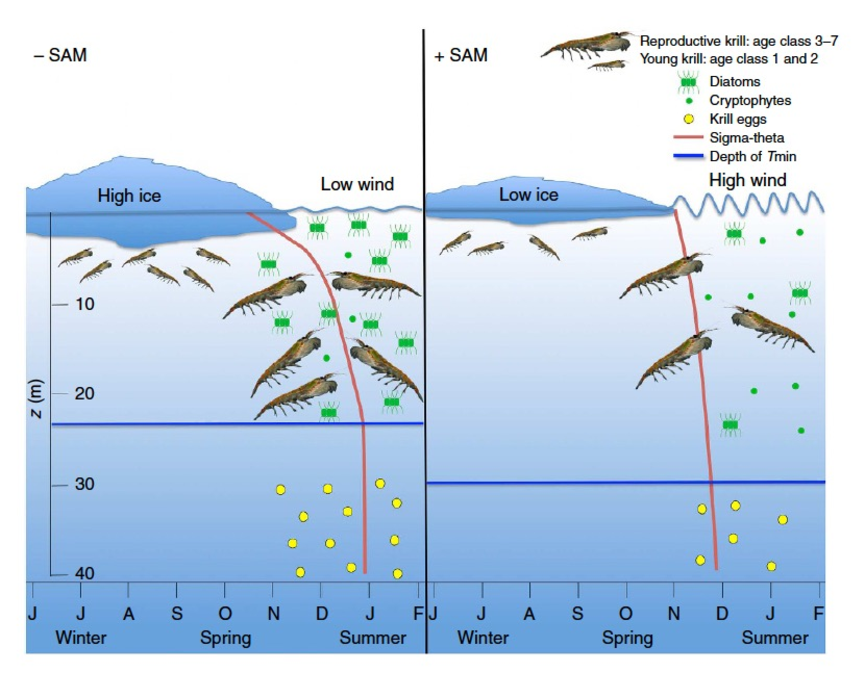
\includegraphics[width=0.7\linewidth]{images/Krill} 

}

\caption{Impactos del SAM en la productividad primaria del Océano Austral (Saba et al. 2013)}\label{fig:unnamed-chunk-4}
\end{figure}

Otro fenómeno oceanográfico-atmosférico que también tiene implicancias
en los océanos es la Oscilación del Sur El Niño, que en inglés es El
Niño Southern Oscilation (ENSO, por sus siglas en inglés). Un evento
``El Niño'' consiste principalmente en un calentamiento por sobre lo
normal de la superficie del Océano Pacífico ecuatorial central y
oriental (mayor a 25ºC), acompañado por un aumento del nivel del mar
(mayor a 15 cm.). Estos eventos que afectan a todo el Océano Pacífico,
incluso llegando los efectos demostrados al Océano Austral, se presentan
en forma cíclica pero a intervalos de tiempo irregulares que fluctúan
entre períodos de dos y diez años. El fenómeno se inicia en el Océano
Pacífico tropical, cerca de Australia e Indonesia, alterándose con ello
la presión atmosférica en zonas muy distantes entre sí, hay cambios en
la dirección y en la velocidad de los vientos, así como el
desplazamiento de las zonas de lluvia a la región tropical. En
condiciones normales, también llamadas condiciones No-Niño, los vientos
alisios (que soplan de este a oeste) acumulan una gran cantidad de agua
y calor en la parte occidental de este océano. El nivel superficial del
mar es, en consecuencia, aproximadamente medio metro más alto en
Indonesia que frente a las costas del Perú y Ecuador. Además, la
diferencia en la temperatura superficial del mar es de alrededor de 8ºC.
entre ambas zonas del Pacífico. Las temperaturas frías se presentan en
América del Sur por que suben las aguas profundas y producen una agua
rica en nutrientes que mantiene el ecosistema marino, y dentro de esto
se sustentan las grandes pesquerías pelágicas (anchoveta y sardina). Las
condiciones No-Niño América del Sur implica un clima atmosférico
relativamente seco.

En cambio durante el fenómeno de El Niño los vientos alisios se
debilitan o dejan de soplar, la máxima temperatura marina se desplaza
hacia la Corriente de Perú que es relativamente fría y la mínima
temperatura marina se desplaza hacia el Sureste Asiático. Esto provoca
el aumento de la presión atmosférica en el sureste asiático y la
disminución en América del Sur. Todo este cambio ocurre en un intervalo
de seis meses, aproximadamente desde junio a noviembre.

Una abundante y bien documentada literatura apoya la tesis que las
fluctuaciones en el ambiente marino por efecto de fenómenos climáticos
como El Niño tienen un notable impacto en poblaciones marinas, en
diferentes escalas de tiempo y espacio. Para evaluar los efectos de este
fenómeno en las zona centro-sur de las costas de Chile, el trabajo de
Arcos et al. (\protect\hyperlink{ref-Arcos2004}{2004}), abordó los
impactos en pesquerías pelágicas de la zona centro-sur de Chile, en
donde se identificaron los cambios de la estructura de la población de
jurel \emph{Trachurus symmetricus}, haciendo colapsar a la industria
pesquera, en lo que se conoce como la ``Crisis del 97'' (Arcos et al.,
\protect\hyperlink{ref-Arcos2004}{2004}).

Uno de los principales efectos del fenómeno El Niño que esgrime el
trabajo de Arcos et al. (\protect\hyperlink{ref-Arcos2004}{2004}) es que
la población juvenil del jurel ``se acorraló'' en el sector centro-sur
(zona de intensa pesquería) por efecto de las malas condiciones de las
aguas del norte (mas cálidas durante El Niño). Esto tuvo como
consecuencia una explotación intensa de individuos de menos de 26 cm.
(juveniles), con lo cual no se pudo regenerar el stock comercial los
años posteriores disminuyendo los desembarques y provocando estragos por
todos conocidos. La Figura 5 representa un modelo conceptual de las
poblaciones de jurel bajo condiciones normales del océano (izquierda) y
frente a una condición El Niño (derecha).

\begin{figure}

{\centering 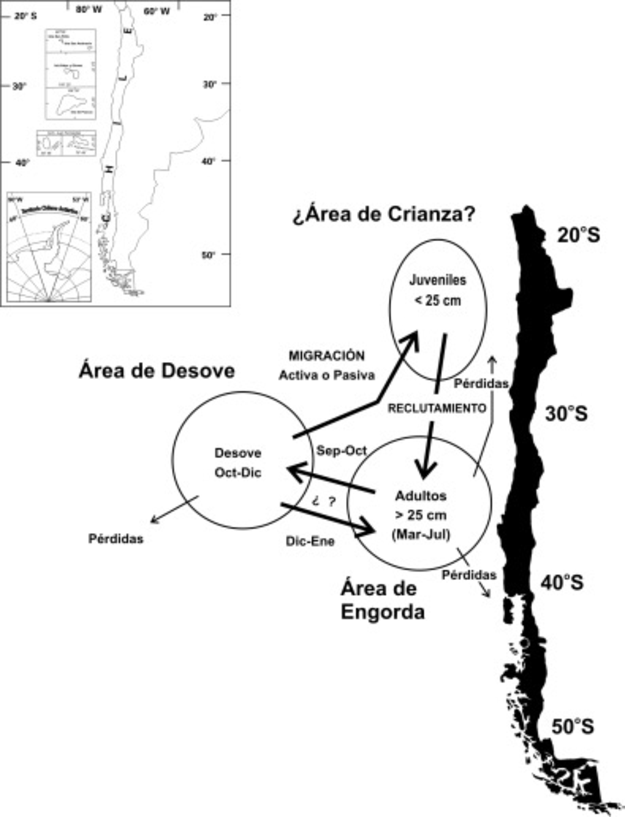
\includegraphics[width=0.45\linewidth,height=0.4\textheight]{images/Exa11} 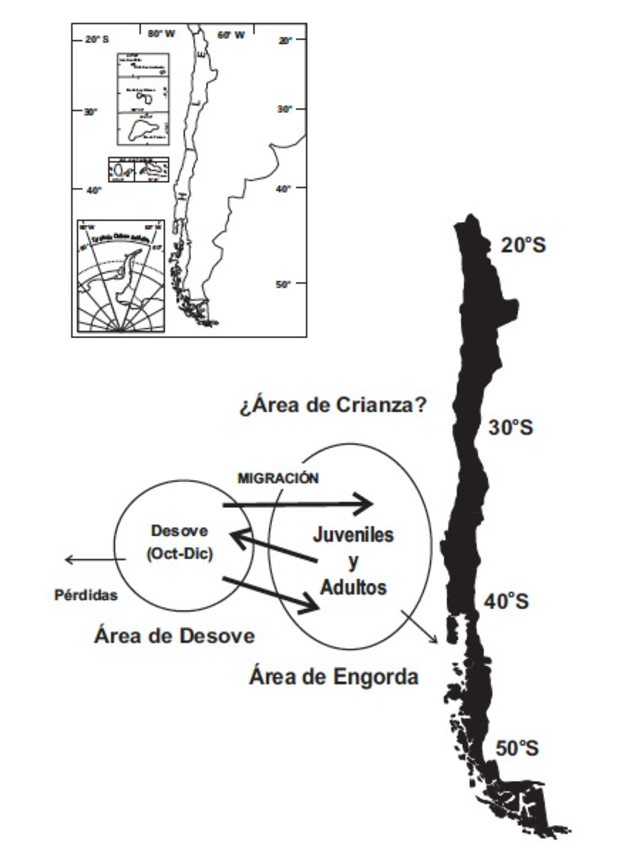
\includegraphics[width=0.45\linewidth,height=0.4\textheight]{images/Exa12} 

}

\caption{Modelo conceptual del impacto de las condiciones no Niño (izq.) y Niño (der.) sobre las poblaciones de jurel en las costas de Chile (Arcos et al. 2004)}\label{fig:unnamed-chunk-5}
\end{figure}

El CC ha generado desjustes temporales de fenómenos
oceanográfico-atmosféricos que moldean a las poblaciones marinas en los
océanos del hemisferio Sur, como son el ENSO y SAM (Lovenduski \&
Gruber, \protect\hyperlink{ref-Lovenduski2005}{2005}; Morley et al.,
\protect\hyperlink{ref-Morley2020}{2020}; Saba et al.,
\protect\hyperlink{ref-Saba2014}{2014}). Si bien las poblaciones marinas
han tratado de adaptarse y sincronizarse a estos fenómenos
interdecadales, cualquier otro factor natural que esté en juego, como el
calentamiento global, se traducirá en la pérdida de sincronía entre
óptimos ambientales y productividad biológica de estas especies,
causando drásticos cambios a nivel de fisiología, distribución y
productividad. Barange et al.
(\protect\hyperlink{ref-Barange2014}{2014}) identificaron cambios en el
uso de hábitat de poblaciones de sardina y anchovetas en el Golfo de
California y Perú, zonas afectadas por el ENSO. Estas especies alternan
sincrónicamente en relación a sus biomasas, y desacoples producidos por
el CC, ha generado pérdida de ajuste a las condiciones climáticas
óptimas de sus poblaciones.

Si bien existe cierta alternancia y conexión entre estos dos fenómenos
oceanográfico-atmosféricos, Ehrnsten et al.
(\protect\hyperlink{ref-Ehrnsten2019}{2019}) plantea que es díficil
testear el efecto de múltiples forzantes a través de un largo gradiente
espacial con estudios empíricos. Sin empbargo, y a pesar de este
problema logístico, la influencia de estos dos factores está ampliamente
demostrada por la comunidad científica internacional.

\hypertarget{cambio-climuxe1tico-en-poblaciones-marinas-del-ocuxe9ano-austral}{%
\subsection{2.4. Cambio Climático en poblaciones marinas del Océano
Austral}\label{cambio-climuxe1tico-en-poblaciones-marinas-del-ocuxe9ano-austral}}

Los cambios en la distribución de poblaciones marinas demuestran que el
calentamiento global está direccionando a las poblaciones marinas hacia
los polos (Parmesan \& Yohe, \protect\hyperlink{ref-Parmesan2003}{2003};
Perry et al., \protect\hyperlink{ref-Perry2005}{2005}), lo cual pone el
foco en los impactos del cambio climático en ecosistemas de altas
latitudes y sus estructuras comunitarias y poblacionales.

Si bien este tipo de análisis se han realizado con énfasis en los
océanos alrededor del mundo, aún persisten dudas sobre el efecto de los
forzantes anteriormente descritos en poblaciones marinas en ecosistemas
de altas latitudes, y más específicamente en el Océano Austral. Estas
dudas han tratado de ser resueltas, y varios estudios han abordado esta
problemática en especies antárticas y su correlación con forzantes
climáticas y oceanográficas en este tipo de ambientes.

Las tendencias de la temperatura son muy variables en todo el continente
antártico y su océano adyacente, y se ha producido un calentamiento
rápido principalmente sobre la Península Antártica, que se destaca como
una región clara y consistente de rápidos cambios, mientras que las
condiciones han sido mucho más variables en otros sectores (Turner et
al., \protect\hyperlink{ref-Turner2005}{2005}). En algunos casos los
efectos del CC tienen un impacto que tiene una correlación positiva en
el aumento de los indicadores. Pinkerton et al.
(\protect\hyperlink{ref-Pinkerton2021}{2021}) identificaron los impactos
que tiene el cambio de las condiciones climáticas en los productores
primarios (fitoplancton) en los últimos 20 años en el Océano Austral,
identificando un incremento en la mayoría de biomasas de productires
primarios en el OA. Este efecto positivo sobre estas variables se
produciría por el aumento de nutrientes derivados de procesos como
mezcla de la columna de agua, ingreso de polvo marino a capas
subsuperficiales, y derretimiento del casquete de hielos.

El cambio climático está alterando rápidamente el hábitat del krill
antártico \emph{Euphausia superba}, al punto de diezmar sus poblaciones
(Krüger et al., \protect\hyperlink{ref-Kruger2021}{2021}). Esta especie
constituye un factor clave de la red trófica del Océano Austral, al
mismo tiempo que sostiene una pesca comercial de proporciones mundiales
(Atkinson et al., \protect\hyperlink{ref-Atkinson2009}{2009}). El doble
papel del cambio climático forzado y la variabilidad natural que afecta
al hábitat del krill antártico y, por tanto, a la productividad de esta
especie, complica la interacción de cualquier tendencia observada
empirícamente y contribuyen a la incertidumbre en las proyecciones
futuras para un manejo pesquero adecuado (Sylvester et al.,
\protect\hyperlink{ref-Sylvester2021}{2021}).

Las especies objetivo de las pesquerías antárticas actuales incluyen al
bacalao y bacalao antártico \emph{Dissostichus eleginoides} y \emph{D.
mawsoni}. Ambas especies son vulnerables a la sobrepesca debido al
crecimiento lento, la madurez tardía y la fecundidad baja. Esta
vulnerabilidad natural podría aumentar, ya que las comunidades que viven
en el ecosistema antártico también se enfrentan actualmente a
alteraciones de su entorno debido al cambio climático, como el aumento
de la temperatura del agua y la disminución del hielo marino. Estos
peces polares (Notothenioidei) están bien adaptados a las condiciones
ambientales frías del Océano Austral, por lo que cualquier cambio en las
condiciones del medio en que habitan, tednría drásticas consecuencias en
sus niveles poblacionales (Mintenbeck,
\protect\hyperlink{ref-Mintenbeck2017}{2017}). El CC no tiene un impacto
uniforme alrededor de la Antártica, dado que en algunas áreas se prevén
efectos negativos sobre las poblaciones de peces y la supervivencia, los
hábitats e indirectamente sobre los ecosistemas (Vanderhaven,
\protect\hyperlink{ref-Vanderhaven2013}{2013}). En este sentido, y de
acuerdo a (Hidalgo et al., \protect\hyperlink{ref-Hidalgo2011}{2011}),
los efectos sinérgicos de la pesca, el clima y la dinámica interna de
las fluctuaciones de la población son poco entendidos debido a la
complejidad de estas interacciones, más aún en una condición de cambio.

\pagebreak

\hypertarget{discusiuxf3n}{%
\subsection{3. DISCUSIÓN}\label{discusiuxf3n}}

Como se expuso anteriormente, existe profusa evidencia científica que
demuestra que los efectos del Cambio Climático en el océano tendrán
impactos severos y alterarán la vida en los ecosistemas marinos. Es
esencial entonces comprender cuales son los principales factores que
inciden directamente en la estructura, distribución y variables como
biomasa y/o abundancia de las poblaciones marinas alrededor del mundo,
con énfasis en regiones y ecosistemas de altas latitudes como el Océano
Austral.

El Océano Austral es un ecosistema moldeado por las condiciones extremas
a las que está expuesto, y por ello, sus poblaciones se han adaptado
fisiológicamente a estas condiciones. En un escenario de calentamiento
global y variabilidad de condiciones oceanográficas, expone a estas
especies a una vulnerabilidad frente a cambios mínimos de los forzantes
analizados. De acuerdo a lo analizado, cabe destacar que no existen
patrones generales, dado que cada población y cada ecosistema tiene
particularidades que resultarían en variadas respuestas frente a un
mismo forzante. Es por ello que la investigación científica tiene que
hacer el esfuerzo de cubrir la mayor cantidad de especies, así como
también, cada ecosistema para obtener respuestas verosímiles respecto a
los efectos en las poblaciones marinas. De esta forma, la comprensión de
los impactos del CC, así como también sus proyecciones podrían ser mejor
entendidas y a su vez estar mejor preparados para el futuro.

Debemos considerar que el Océano Austral y alrededores es rico y
productivo en vida marina, incluidas especies de moluscos, crustáceos y
peces de interés para la industria pesquera (Arana et al.,
\protect\hyperlink{ref-Arana2020b}{2020}), y actualmente son especies
proclives a cambios en sus dinámicas poblacionales, y si bien, no es
posible determinar si estos cambios del entorno tendrán efectos en la
variabilidad poblacional, el manejo de estas pesquerías debe tener en
cuenta los impactos directos sobre los peces que capturan. Se debería
considerar también áreas específicas de vulnerabilidad de las especies y
el ecosistema marino antártico. Un pequeño cambio de las condiciones
climáticas podría causar un colapso poblacional en las especies
explotadas o en alguna otra especie asociada en su red trófica y
ecológica.

Como señalamos anteriormente, el krill y el bacalao son especies que
habitan el OA y que constituyen importantes pesquerías explotadas por un
conjunto de flotas de distintos paises. En este sentido, hay que
entender y anticiparse a los impactos que tendrán los forzantes sobre
estas poblaciones, y de esta forma ser precautorios y adaptativos en la
extracción y explotación de recursos frente a esas nuevas condiciones
climáticas. Esto puede significar que las cuotas se reduzcan, o que las
asignaciones de captura espaciales y/o temporales sean más explícitas.
Afortunadamente hoy existe un esfuerzo global con varios organismos e
instituciones internacionales que además de cautelar la sustentabilidad
de las pesquerías antes citadas, están haciendo esfuerzos de
investigación tratando de entender los impactos del CC en este océano,
entre ellas, el Comité Científico de Investigaciones Antárticas (SCAR),
el Consejo de Administradores de Programas Antárticos Nacionales
(COMNAP), Asociación Internacional de Operadores Turísticos Antárticos
(IAATO) y Comisión para la Conservación de los Recursos Vivos Marinos
Antárticos (CCAMLR). En este contexto, hoy se desarrollan programas
científicos que intentan lidiar con este desafío del conocimiento, pero
las herramientas analíticas y conceptuales aún tienen que mejorar, dado
que se deben integrar los más variados componentes que influyen en el
CC. Sin embargo, en aspectos relacionados al manejo y evaluación de
estas poblaciones, las preguntas siguen abiertas y en continuo
desarrollo científico tratando de proyectar los impactos que tiene en un
contexto ecosistémico y de cambios climáticos fluctuantes, y cómo ello
afecta a las poblaciones marinas del Océano Austral.

De acuerdo a esta revisión, existen forzantes directos e indirectos como
la temperaratura, oxígeno y procesos oceanografico-atmosfericos como el
SAM y ENSO que tienen impactos directas sobre las poblaciones marinas
del Océano Austral. En este sentido, cambios en los niveles y tendencias
de estos forzantes alterarán funciones tales como la distribución
espacial, ecología y fisiología de las especies que habitan en el Océano
Austral.

\pagebreak

\hypertarget{referencias}{%
\subsection*{4. REFERENCIAS}\label{referencias}}
\addcontentsline{toc}{subsection}{4. REFERENCIAS}

\hypertarget{refs}{}
\begin{cslreferences}
\leavevmode\hypertarget{ref-Arana2020b}{}%
Arana, P. M., Rolleri, R., \& De Caso, Á. (2020). Chilean antarctic
krill fishery (2011-2016). \emph{Latin American Journal of Aquatic
Research}, \emph{48}(2), 179--196.
\url{https://doi.org/10.3856/vol48-issue2-fulltext-2408}

\leavevmode\hypertarget{ref-Arcos2004}{}%
Arcos, D., Cubillos, L., \& Núñez, S. (2004). Efectos de El Niño
1997-1998 sobre las principales pesquerías pelágicas de la zona
centro-sur de Chile . In \emph{S. AVARIA, j. CARRASCO, j. RUTLLANT y e.
YÁÑEZ. (Eds.). 2004. CONA} (pp. 153--177).

\leavevmode\hypertarget{ref-Atkinson2009}{}%
Atkinson, A., Siegel, V., Pakhomov, E. A., Jessopp, M. J., \& Loeb, V.
(2009). A re-appraisal of the total biomass and annual production of
Antarctic krill. \emph{Deep-Sea Research Part I: Oceanographic Research
Papers}, \emph{56}(5), 727--740.
\url{https://doi.org/10.1016/j.dsr.2008.12.007}

\leavevmode\hypertarget{ref-Barange2014}{}%
Barange, M., Merino, G., Blanchard, J. L., Scholtens, J., Harle, J.,
Allison, E. H., Allen, J. I., Holt, J., \& Jennings, S. (2014). Impacts
of climate change on marine ecosystem production in societies dependent
on fisheries. \emph{Nature Climate Change}, \emph{4}(3), 211--216.
\url{https://doi.org/10.1038/nclimate2119}

\leavevmode\hypertarget{ref-Bindoff2019}{}%
Bindoff, N. L., Cheung, W. W. L., Kairo, J. G., Arístegui, J., Guinder,
V. A., Hallberg, R., Hilmi, N., Jiao, N., Karim, M. S., Levin, L.,
O'Donoghue, S., Cuicapusa, S. R. P., Rinkevich, B., Suga, T., Tagliabue,
A., \& Williamson, P. (2019). Changing Ocean, Marine Ecosystems, and
Dependent Communities. In: IPCC Special Report on the Ocean and
Cryosphere in a Changing Climate. In \emph{IPCC special report on the
ocean and cryosphere in a changing climate} (pp. 447--588).

\leavevmode\hypertarget{ref-Bryndum-Buchholz2019}{}%
Bryndum-Buchholz, A., Tittensor, D. P., Blanchard, J. L., Cheung, W. W.
L., Coll, M., Galbraith, E. D., Jennings, S., Maury, O., \& Lotze, H. K.
(2019). Twenty-first-century climate change impacts on marine animal
biomass and ecosystem structure across ocean basins. \emph{Global Change
Biology}, \emph{25}(2), 459--472.
\url{https://doi.org/10.1111/gcb.14512}

\leavevmode\hypertarget{ref-Cheung2010a}{}%
Cheung, W. W. L., Lam, V. W. Y., Sarmiento, J. L., Kearney, K., Watson,
R., Zeller, D., \& Pauly, D. (2010). Large-scale redistribution of
maximum fisheries catch potential in the global ocean under climate
change. \emph{Global Change Biology}, \emph{16}(1), 24--35.
\url{https://doi.org/10.1111/j.1365-2486.2009.01995.x}

\leavevmode\hypertarget{ref-Cheung2013}{}%
Cheung, W. W. L., Sarmiento, J. L., Dunne, J., Frölicher, T. L., Lam, V.
W. Y., Palomares, M. L., Watson, R., \& Pauly, D. (2013). Shrinking of
fishes exacerbates impacts of global ocean changes on marine ecosystems.
\emph{Nature Climate Change}, \emph{3}(3), 254--258.
\url{https://doi.org/10.1038/nclimate1691}

\leavevmode\hypertarget{ref-Deutsch2015}{}%
Deutsch, C., Ferrel, A., Seibel, B., Pörtner, H.-O., \& Raymond B. Huey.
(2015). Constraint on Marine Habitats. \emph{Science}, \emph{348}(6239),
1132--1136.

\leavevmode\hypertarget{ref-Duncan2020}{}%
Duncan, M. I., James, N. C., Potts, W. M., \& Bates, A. E. (2020).
Different drivers, common mechanism; the distribution of a reef fish is
restricted by local-scale oxygen and temperature constraints on aerobic
metabolism. \emph{Conservation Physiology}, \emph{8}(1).
\url{https://doi.org/10.1093/conphys/coaa090}

\leavevmode\hypertarget{ref-Ehrnsten2019}{}%
Ehrnsten, E. S., Bauer, B., \& Gustafsson, B. G. (2019). Combined
effects of environmental drivers on marine trophic groups - A systematic
model comparison. \emph{Frontiers in Marine Science}, \emph{6}(JUL),
1--14. \url{https://doi.org/10.3389/fmars.2019.00492}

\leavevmode\hypertarget{ref-Frawley2019}{}%
Frawley, T. H., Briscoe, D. K., Daniel, P. C., Britten, G. L., Crowder,
L. B., Robinson, C. J., Gilly, W. F., \& Arkhipkin, A. (2019). Impacts
of a shift to a warm-water regime in the Gulf of California on jumbo
squid (Dosidicus gigas). \emph{ICES Journal of Marine Science},
\emph{76}(7), 2413--2426. \url{https://doi.org/10.1093/icesjms/fsz133}

\leavevmode\hypertarget{ref-Hidalgo2018}{}%
Hidalgo, M., Mihneva, V., Vasconcellos, M., \& Bernal, M. (2018).
\emph{Impact of Climate Change on Fisheries and Aquaculture} (Vol. 627,
pp. 113--138).

\leavevmode\hypertarget{ref-Hidalgo2011}{}%
Hidalgo, M., Rouyer, T., Molinero, J. C., Massutí, E., Moranta, J.,
Guijarro, B., \& Stenseth, N. C. (2011). Synergistic effects of
fishing-induced demographic changes and climate variation on fish
population dynamics. \emph{Marine Ecology Progress Series},
\emph{426}(April 2014), 1--12. \url{https://doi.org/10.3354/meps09077}

\leavevmode\hypertarget{ref-IPCC2014}{}%
IPCC. (2014). \emph{Climate Change 2014: Synthesis Report. Contribution}
(p. 169).

\leavevmode\hypertarget{ref-Isensee2016}{}%
Isensee, K., Levin, L. A., Breitburg, D., Gregoire, M., Veronique, G.,
\& Valdes, L. (2016). The Ocean is Losing its Breath. \emph{Ocean and
Climate Scientific Notes}, \emph{ed 2}, 20--31.
\url{www.ocean-climate.org}

\leavevmode\hypertarget{ref-Koenigstein2016}{}%
Koenigstein, S., Mark, F. C., Gößling-Reisemann, S., Reuter, H., \&
Poertner, H. O. (2016). Modelling climate change impacts on marine fish
populations: process-based integration of ocean warming, acidification
and other environmental drivers. \emph{Fish and Fisheries},
\emph{17}(4), 972--1004. \url{https://doi.org/10.1111/faf.12155}

\leavevmode\hypertarget{ref-Kortsch2015}{}%
Kortsch, S., Primicerio, R., Fossheim, M., Dolgov, A. V., \& Aschan, M.
(2015). Climate change alters the structure of arctic marine food webs
due to poleward shifts of boreal generalists. \emph{Proceedings of the
Royal Society B: Biological Sciences}, \emph{282}(1814).
\url{https://doi.org/10.1098/rspb.2015.1546}

\leavevmode\hypertarget{ref-Kruger2021}{}%
Krüger, L., Huerta, M. F., Santa Cruz, F., \& Cárdenas, C. A. (2021).
Antarctic krill fishery effects over penguin populations under adverse
climate conditions: Implications for the management of fishing
practices. \emph{Ambio}, \emph{50}(3), 560--571.
\url{https://doi.org/10.1007/s13280-020-01386-w}

\leavevmode\hypertarget{ref-Lovenduski2005}{}%
Lovenduski, N. S., \& Gruber, N. (2005). Impact of the Southern Annular
Mode on Southern Ocean circulation and biology. \emph{Geophysical
Research Letters}, \emph{32}(11), 1--4.
\url{https://doi.org/10.1029/2005GL022727}

\leavevmode\hypertarget{ref-Marshall2018}{}%
Marshall, A. G., Hemer, M. A., Hendon, H. H., \& McInnes, K. L. (2018).
Southern annular mode impacts on global ocean surface waves. \emph{Ocean
Modelling}, \emph{129}(October 2020), 58--74.
\url{https://doi.org/10.1016/j.ocemod.2018.07.007}

\leavevmode\hypertarget{ref-Melbourne-Thomas2021}{}%
Melbourne-Thomas, J., Audzijonyte, A., Brasier, M. J., Cresswell, K. A.,
Fogarty, H. E., Haward, M., Hobday, A. J., Hunt, H. L., Ling, S. D.,
McCormack, P. C., Mustonen, T., Mustonen, K., Nye, J. A., Oellermann,
M., Trebilco, R., Putten, I. van, Villanueva, C., Watson, R. A., \&
Pecl, G. T. (2021). Poleward bound: adapting to climate-driven species
redistribution. \emph{Reviews in Fish Biology and Fisheries}, \emph{3}.
\url{https://doi.org/10.1007/s11160-021-09641-3}

\leavevmode\hypertarget{ref-Mintenbeck2017}{}%
Mintenbeck, K. (2017). Impacts of Climate Change on the Southern Ocean.
In \emph{Climate change impacts on fisheries and aquaculture}.
\url{https://doi.org/10.1002/9781119154051.ch20}

\leavevmode\hypertarget{ref-Morley2020}{}%
Morley, S. A., Abele, D., Barnes, D. K. A., Cárdenas, C. A., Cotté, C.,
Gutt, J., Henley, S. F., Höfer, J., Hughes, K. A., Martin, S. M.,
Moffat, C., Raphael, M., Stammerjohn, S. E., Suckling, C. C., Tulloch,
V. J. D., Waller, C. L., \& Constable, A. J. (2020). Global Drivers on
Southern Ocean Ecosystems: Changing Physical Environments and
Anthropogenic Pressures in an Earth System. \emph{Frontiers in Marine
Science}, \emph{7}(December), 1--24.
\url{https://doi.org/10.3389/fmars.2020.547188}

\leavevmode\hypertarget{ref-Parmesan2003}{}%
Parmesan, C., \& Yohe, G. (2003). A globally coherent fingerprint of
climate change impacts across natural systems. \emph{Nature},
\emph{421}(6918), 37--42. \url{https://doi.org/10.1038/nature01286}

\leavevmode\hypertarget{ref-Perry2005}{}%
Perry, A. L., Low, P. J., Ellis, J. R., \& Reynolds, J. D. (2005).
Ecology: Climate change and distribution shifts in marine fishes.
\emph{Science}, \emph{308}(5730), 1912--1915.
\url{https://doi.org/10.1126/science.1111322}

\leavevmode\hypertarget{ref-Pinkerton2021}{}%
Pinkerton, M. H., Boyd, P. W., Deppeler, S., Hayward, A., Höfer, J., \&
Moreau, S. (2021). Evidence for the Impact of Climate Change on Primary
Producers in the Southern Ocean. \emph{Frontiers in Ecology and
Evolution}, \emph{9}(May), 1--19.
\url{https://doi.org/10.3389/fevo.2021.592027}

\leavevmode\hypertarget{ref-Pinsky2020}{}%
Pinsky, M. L., Selden, R. L., \& Kitchel, Z. J. (2020). Climate-Driven
Shifts in Marine Species Ranges: Scaling from Organisms to Communities.
\emph{Annual Review of Marine Science}, \emph{12}, 153--179.
\url{https://doi.org/10.1146/annurev-marine-010419-010916}

\leavevmode\hypertarget{ref-Pinones2016}{}%
Piñones, A., \& Fedorov, A. V. (2016). Projected changes of Antarctic
krill habitat by the end of the 21st century. \emph{Geophysical Research
Letters}, \emph{43}(16), 8580--8589.
\url{https://doi.org/10.1002/2016GL069656}

\leavevmode\hypertarget{ref-Portner2001}{}%
Pörtner, H. (2001). Climate change and temperature-dependent
biogeography: Oxygen limitation of thermal tolerance in animals.
\emph{Naturwissenschaften}, \emph{88}(4), 137--146.
\url{https://doi.org/10.1007/s001140100216}

\leavevmode\hypertarget{ref-Rijnsdorp2009}{}%
Rijnsdorp, A. D., Peck, M. A., Engelhard, G. H., Möllmann, C., \&
Pinnegar, J. K. (2009). Resolving the effect of climate change on fish
populations. \emph{ICES Journal of Marine Science}, \emph{66}(7),
1570--1583. \url{https://doi.org/10.1093/icesjms/fsp056}

\leavevmode\hypertarget{ref-Saba2014}{}%
Saba, G. K., Fraser, W. R., Saba, V. S., Iannuzzi, R. A., Coleman, K.
E., Doney, S. C., Ducklow, H. W., Martinson, D. G., Miles, T. N.,
Patterson-Fraser, D. L., Stammerjohn, S. E., Steinberg, D. K., \&
Schofield, O. M. (2014). Winter and spring controls on the summer food
web of the coastal West Antarctic Peninsula. \emph{Nature
Communications}, \emph{5}. \url{https://doi.org/10.1038/ncomms5318}

\leavevmode\hypertarget{ref-Shoji2011}{}%
Shoji, J., Toshito, S. I., Mizuno, K. I., Kamimura, Y., Hori, M., \&
Hirakawa, K. (2011). Possible effects of global warming on fish
recruitment: Shifts in spawning season and latitudinal distribution can
alter growth of fish early life stages through changes in daylength.
\emph{ICES Journal of Marine Science}, \emph{68}(6), 1165--1169.
\url{https://doi.org/10.1093/icesjms/fsr059}

\leavevmode\hypertarget{ref-Sylvester2021}{}%
Sylvester, Z. T., Long, M. C., \& Brooks, C. M. (2021). Detecting
Climate Signals in Southern Ocean Krill Growth Habitat. \emph{Frontiers
in Marine Science}, \emph{8}(June), 1--15.
\url{https://doi.org/10.3389/fmars.2021.669508}

\leavevmode\hypertarget{ref-Turner2005}{}%
Turner, J., Colwell, S. R., Marshall, G. J., Lachlan-Cope, T. A.,
Carleton, A. M., Jones, P. D., Lagun, V., Reid, P. A., \& Iagovkina, S.
(2005). Antarctic climate change during the last 50 years.
\emph{International Journal of Climatology}, \emph{25}(3), 279--294.
\url{https://doi.org/10.1002/joc.1130}

\leavevmode\hypertarget{ref-Vanderhaven2013}{}%
Vanderhaven, B. (2013). \emph{Effects on Ecosystems and Fisheries
Management} (Vol. 15).

\leavevmode\hypertarget{ref-Veytia2020}{}%
Veytia, D., Corney, S., Meiners, K. M., Kawaguchi, S., Murphy, E. J., \&
Bestley, S. (2020). Circumpolar projections of Antarctic krill growth
potential. \emph{Nature Climate Change}, \emph{10}(6), 568--575.
\url{https://doi.org/10.1038/s41558-020-0758-4}

\leavevmode\hypertarget{ref-Worm2012}{}%
Worm, B., Hilborn, R., Baum, J. K., Branch, T. A., Collie, J. S.,
Costello, C., Fogarty, M. J., Fulton, E. A., Hutchings, J. A., Jennings,
S., Jensen, O. P., Lotze, H. K., Mace, P. M., \& Mcclanahan, T. R.
(2012). \emph{Rebuilding Global Fisheries}. \emph{578}(2009).
\url{https://doi.org/10.1126/science.1173146}
\end{cslreferences}


\newpage
\begin{figure}

\vspace*{1cm}
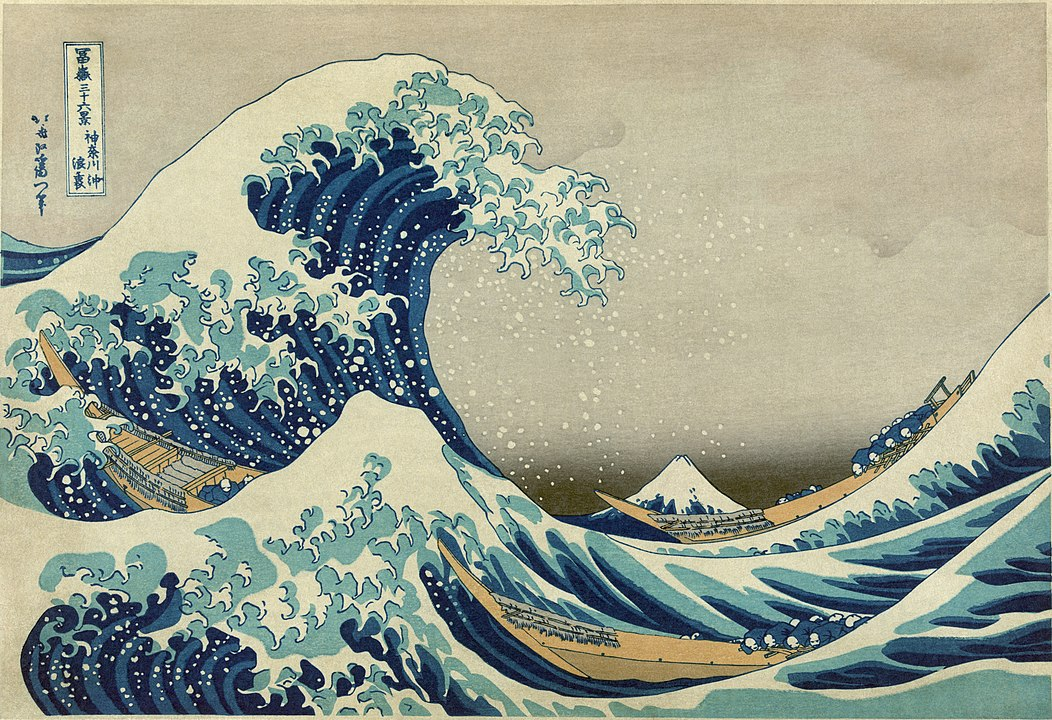
\includegraphics[]{images/Exa16.jpg}

\end{figure}

\vspace*{0.5cm}

\begin{center}
\emph{La gran ola de Kanagawa, del artista japonés Hokusai (c. 1829--1833) ha sido interpretada, entre otras cosas, como una advertencia de la fuerza y el impacto de los cambios abruptos sobre la naturaleza. En el contexto actual, esta pintura nos puede entregar otra mirada y (re)transmitir la fuerza y el impacto que tiene el acelerado Cambio Climático sobre el medio marino, y por ende en la humanidad.}


\end{center}


\end{document}
